\documentclass{article}
\usepackage{arxiv}
\usepackage[utf8]{inputenc} 
\usepackage{float}
\usepackage{listings}
\usepackage[T1]{fontenc}    
\usepackage{hyperref}       
\usepackage{url}            
\usepackage{mathtools}
\usepackage{amssymb,mathrsfs}
\usepackage{booktabs}       
\usepackage{amsfonts}       
\usepackage{dsfont}   
\usepackage[ruled,vlined]{algorithm2e}
\usepackage[spanish]{babel}

\title{El Problema de la Asignación Generalizado}
\author{
  Sandra del Mar Soto Corderi\\
  No. cuenta: 315707267
}
\date{}

\begin{document}
\maketitle

\section{Introducción}

El problema del que se hablará en este reporte es el de asignación generalizada mejor conocido \textbf{GAP}. 

Este es un problema NP conocido que trata de lo siguiente:

Dadas $n$ tareas y $m$ trabajadores o agentes, se quieren asignar todas las tareas a los trabajadores. Cada trabajador tiene cierta energía o $capacidad$ que decrementa conforme se le asignan tareas, cada tarea gasta cierto valor de la $capacidad$, este valor variando dependiendo del trabajador al que se asigne, esto se puede ver como cuanta "dificultad" le puede costar al trabajador realizar la tarea. Además cada tarea tiene un $costo$ que depende del trabajador que la vaya realizar.

La $capacidad$ total del trabajador (b), la capacidad que gasta una tarea dependiendo del trabajador y el $costo$ se pueden ver como las siguientes funciones:
\[capacidadTotal=b(w)\]
\[capacidad=a(t,w)\] 
\[costo=\sum_{t=1}^{n}\sum_{w=1}^{m}c(t,w)\times x(t,w)\]
Donde $w$ es un trabajador, $t$ es una tarea y $x(t,w)$ es la función que 
representa si la tarea $t$ está asignada al trabajador $w$, es decir:
\[x(t,w)=
\begin{cases}
\text{1}&\quad\text{si $w$ realiza la tarea $t$}\\
\text{0}&\quad\text{e.o.c}
\end{cases}\]

Lo que busca optimizar el problema GAP es la función de costo, pero esto no es lo único que se necesita para una solución factible. Una solución es factible si y sólo si se cumplen las siguientes condiciones:
\begin{enumerate}
	\item Toda tarea debe estar asignada a algún trabajador.
	\[\forall t \exists w (x(t,w)=1)\]
	\item Ninguna tarea debe estar asignada al mismo tiempo a dos o más 
	trabajadores.
	\[\forall t \neg \exists w_1,w_2 (x(t,w1)=1 \;\wedge \; x(t,w_2)=1)\]
	\item Un trabajador no debe superar su $capacidadTotal$.
	\[\forall w \left(\sum_{t=1}^{n}a(t,w)\times x(t,w) \; \leq b(j)\right)\]
\end{enumerate}

\subsection{Búsqueda Tabú \emph{(Tabu Search)}}
Ahora hablaremos de la heurística que se utilizó:

Buscando artículos de investigación sobre el problema de asignación generaliza, me encontré con varios que usaban heurística híbridas, en estos híbridos siempre mencionaban a la búsqueda tabú. Un artículo en específico me llamo la atención \cite{gap}. Este artículo describe como resolver el problema usando búsqueda adaptativa. La heurística de búsqueda adaptativa propuesta para resolver el GAP puede ser descrita en una estructura general incluyendo tres fases, que son aplicados repetidamente hasta que algún criterio de parada sea verificado:\\
Fase 1: Generar una solución usando una heurística aleatoria tipo greedy.\\
Fase 2: Aplicar un método de búsqueda local.\\
Fase 3: Actualizar los parámetros (si hay).\\
Más adelante en el artículo explican como la búsqueda tabú entra en estos.

Los artículos \cite{tsgap} y \cite{tshgap} resuelven el problema GAP usando búsqueda tabú y proponen la generación de la solución inicial de forma similar, plantean que como solemos tener más tareas que trabajadores, se puede reducir el problema a knapsack o mejor conocido como problema de la mochila y resolverse con el algoritmo de Martello y Toth (Un algoritmo greedy muy utilizado para problemas de knapsack). 

De todo lo anterior decidí usar un método greedy para obtener mi solución inicial, quise implementar el algoritmo de Martello y Toth, pero consideré era demasiado 

Ahora vamos a explicar de una forma muy sencilla en que consiste la búsqueda tabú:



En este proyecto se uso la versión simplificada, donde no se hace manejo de la memoria a mediano y largo plazo, es decir se siguió un algoritmo muy parecido al que presentan en \cite{clever}. A continuación se muestra el algoritmo usado en el proyecto:

\begin{algorithm}[H]
	\SetAlgoLined
	\KwOut{$S_{mejor}$ mejor solución encontrada}
	\KwIn{La condición de paro $SC$, tamaño máximo de lista tabú $TM$, $S_{inicial}$ una solución inicial}
	$S_{mejor} \leftarrow S_{inicial}$
	$ListaTabu \leftarrow S_{mejor}$
	\While{ $\neg SC$}{
		\For{$S_{candidato} \in Vecindad_s$}{
			\If{$\neg SeEncuentra(S_{candidato}, ListaTabu)$}{
			$ListaCandidatos \leftarrow S_{candidato}$}
		}
		$S_{candidato} \leftarrow BuscaMejorCandidato(ListaCandidatos)$\\
		\If{$Costo(S_{candidato}) \leq Costo(S_{mejor})$}{
			$S_{mejor} \leftarrow S_{candidato}$\\
			$ListaTabu \leftarrow S_{candidato}$
		}
		\While{$ListaTabu > TM$}{
			$EliminaPrimer(ListaTabu)$
		}
	}
	\Return{$S_{mejor}$}
	\caption{Búsqueda Tabú simplificada}
\end{algorithm}

\section{Tecnologías usadas en el programa}
\begin{itemize}
	\item{ \textbf{Lenguaje de programación:} Kotlin 1.4.10. 
		
	Este proyecto se inició en el lenguaje de programación Rust pero por problemas de configuración y por cuestiones de tiempo, se decidió cambiar a un lenguaje ya conocido como es Java, pero ya que el profesor no es muy aficionado a Java, se buscaron alternativas y la mejor opción encontrada en ese momento fue Kotlin. Kotlin tiene una sintaxis muy intuitiva y permite usar todas las bibliotecas de Java.}
	\item {\textbf{IDE:} IntelliJ IDEA
		
	Es la IDE más popular para Java y es compatible con Kotlin, por lo que se usó}
	\item {\textbf{Sistema de construcción:} Gradle 6.7
		
	Al investigar la documentación de Kotlin, se mencionaba a Gradle y a Maven como las mejores opciones para usar como sistema de construcción. Gradle tenía el tutorial más corto, así como manejaba las dependencias más fácilmente que Maven, por ello se escogió.
	}
	\item {\textbf{Documentación:} dokkaHtml 1.4.10.2  
	
	Es el sistema de documentación oficial de Kotlin}
	\item {\textbf{Graficación:} Gnuplot 5.0}
	\item {\textbf{Insumos:} Los insumos (datos de entrada) fueron proporcionados por el profesor Victor mediante una base de datos relacional \textit{SQL}. El sistema manejador de la base de datos utilizado es SQLite 3.16.2. El controlador del \textit{SMBD} es una biblioteca para Kotlin SQLite-JDBC 3.28.0.}
	\item {\textbf{Control de versiones:} Para mantener el control de versiones se utilizó Git 2.17.1 y el repositorio en línea se encuentra alojado en GitHub.}
\end{itemize}

\section{Diseño del programa}

\begin{figure}[H]
	\centering
	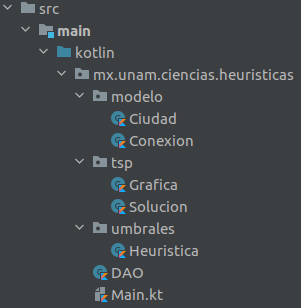
\includegraphics[scale=0.8]{imgs/estructura.png}
	\caption{Estructura de las clases del proyecto}
\end{figure}

El proyecto se hizo con un enfoque orientado a objetos, por la naturaleza del lenguaje escogido. 

Originalmente se iban a generar varias interfaces, pero al final se optó por un diseño más sencillo: El proyecto se dividió en tres paquetes: 
\begin{itemize}
	\item modelo
	
	En este paquete se crean los objetos que estaremos manejando en el proyecto y cuya información no cambiará, como son los valores de las tareas, los trabajadores, el costo de sus asignaciones y las capacidades necesarias.
	
	\item gap
	
	En este paquete tenemos todos los métodos o funciones necesarios para resolver el problema de gap sin aplicar la heurística
	
	\item tabu
	
	En este paquete tenemos los métodos o funciones necesarios para aplicar la heurística de búsqueda tabú al problema anterior.
\end{itemize}


A continuación se van a enlistar las clases usadas y lo que hace cada una:
\begin{itemize}
	\item {Tarea.kt
		
		Esta clase almacena la información de las ciudades de nuestro problema, es decir, las coordenadas, nombre, id, población, de cada ciudad que se usará en el problema. Se declaró como una \emph{data class} de Kotlin, ya que este tipo de clases se dedican únicamente a almacenar información, lo que hace que al construir el objeto, hayan varios métodos ya implementados. Igualmente es necesario comentar que no se incluyó la implementación de getters y setters debido a que en Kotlin en la documentación mencionan que no son necesarios.
	}
	\item {Trabajador.kt
		
		Esta clase es análoga a la de Ciudad en la cuestión que es una \emph{data class} donde guardamos las conexiones entre ciudades. Originalmente no se iba a usar este objeto, pero para facilitar el acceso a la base de datos con el DAO, se creó.
	}
	\item {Grafica.kt
		
		Esta clase es de las que cuentan con más métodos y es donde se realizan todas las funciones de la gráfica. Nuestra gráfica se representa como una matriz de adyacencia cuya forma de llenado sigue la definición de peso aumentado mencionado en la introducción. En esta clase se manejan los objetos de ciudad y conexion para obtener la información necesaria de acuerdo a la función. Cabe mencionar que para optimizar el tiempo en que corre el programa se agregó una función para obtener el peso de forma más directa, esta función optimiza la obtención del costo de la instancia una vez que se hace intercambio de índices al tomar las 4 aristas posibles de la gráfica que se ven afectadas con este intercambio y así obtener el nuevo costo restando los pesos de estas aristas eliminadas y la suma de agregar los nuevas aristas. Así obtenemos el peso durante las soluciones de forma constante y no lineal como sería en el caso de mandar a llamar a la función de costo de nuevo en cada caso.
	}
	\item {Solucion.kt
		
		Esta clase es bastante sencilla, ya que solo crea soluciones para el tsp, es decir invierte aleatoriamiente vecinos de la ruta para crear nuevas con la esperanza de que mejore. Esta clase originalmente iba a ir integrada con la clase de Grafica, pero era más limpio y fácil de comprender manejar los métodos de la clase heuristica con un objeto sencillo Solucion que con el objeto de una clase llena de métodos como es Grafica.
	
	}
	\item {Heuristica.kt
		
		Esta podría considerarse como la clase más ilustrativa del objetivo de este proyecto ya que es la que realiza el procedimiento de la heurística de recocido simulado con aceptación por umbrales. En pocas palabras el procedimiento que se sigue es obtener una temperatura con un valor lo suficientemente grande como para recorrer el espacio de búsqueda de forma rápida, esta temperatura se va disminuyendo al multiplicarla con un factor de congelamiento y mientras se enfría se van generando soluciones nuevas, de las cuales se toman las mejores. Los métodos de esta clase son la implementación los algoritmos que vienen descritos en el pdf llamado hoc que se encuentra dentro de la carpeta fuentes en este mismo directorio. Se había implementado un método que optimizaba los resultados, este método revisaba todos los vecinos de la mejor solución y tomaba el mejor de ellos, pero alentaba tanto al sistema que no se podían hacer las pruebas con muchas semillas.
	
	}
	\item {DAO.kt
		
		Esta clase funciona como nuestro Data Access Object, es la clase que se conecta con la base de datos directamente. Usamos un DAO por nuestro diseño basado en orientación a objetos y para mantener el patrón Modelo-Controlador. Normalmente los DAO no se aconsejan para aplicaciones donde el tiempo de ejecución importa pero es mucho más eficiente tener que hacer una o dos consultas a la base de datos mediante el DAO que hacer varias consultas dentro del modelo.
	}
	\item {Main.kt
		
		Este archivo no es una clase como tal, sino es el main donde se ejecuta el sistema. Lo que hace es tomar la lista de ciudades dada por el usuario con las cuales crea un objeto gráfica, este objeto gráfica manda a crear soluciones usando el rango de semillas proporcionado y manda a llamar a la heurística para mejorar la solución en los parámetros que se den. Al final se imprimen los costos de todas las mejores soluciones y se regresa la ruta de la mejor solución de todas.
	}
\end{itemize}

Para ver más detalladamente la implementación, favor de generar la documentación con dokkahtml.


\section{Resultados}

Probando diferentes semillas de un lote con varias semillas para todas las instancias de GAP, se logró encontrar una semilla para cada ejemplar de forma que se obtuvieran soluciones factibles y se tomó la mejor solución de todas.

El sistema tiene la cualidad de que cada vez que lo ejecutas aunque sea con la misma semilla, no te dará la misma función de costo, esto es por como se implementó la aleatoriedad en las soluciones dentro del programa. Por esa razón siempre se devuelve la asignación de la mejor solución, para que no se pierda. 

Los parámetros usados en el sistema de la heurística fueron cambiando de acuerdo a pruebas hechas con pocas semillas y las recomendaciones del profesor y la clase, después de encontrar mejores soluciones satisfactorias, los parámetros quedaron de la siguiente forma:
\begin{itemize}
\item Límite superior para las iteraciones o mejor dicho, la condición de paro
L = 20000
\item Número máximo de iteraciones para calcular vecinos 
numTareas * 10
\item Tamaño máximo que puede tener la lista tabú
L = 100
\end{itemize}

\subsection{Instancia con 500 trabajadores (db)}

El sistema tarda un aproxima de 45 a 55 minutos para correr esta instancia con una semilla.

Por ello solo se probaron 5 semillas, esto tardó 5h 13m 52s y se obtuvieron los siguientes resultados:

Mejor Semilla: 2\\
Mejor Costo: 2346.536428458342\\
\begin{lstlisting}
Trabajador 1 -> Tarea:149 , Tarea:213 , Tarea:310 , Tarea:953 , 
Trabajador 2 -> Tarea:341 , Tarea:399 , Tarea:495 , 
Trabajador 3 -> Tarea:737 , 
Trabajador 4 -> Tarea:578 , Tarea:580 , Tarea:598 , Tarea:778 , 
Trabajador 5 -> Tarea:101 , Tarea:764 , 
Trabajador 6 -> Tarea:311 , Tarea:489 , 
Trabajador 7 -> Tarea:889 , 
Trabajador 8 -> Tarea:723 , Tarea:908 , 
Trabajador 9 -> Tarea:484 , Tarea:586 , Tarea:903 , Tarea:943 , 
Trabajador 10 -> 
Trabajador 11 -> Tarea:964 , 
Trabajador 12 -> Tarea:148 , Tarea:661 , Tarea:742 , Tarea:885 , 
Trabajador 13 -> 
Trabajador 14 -> Tarea:423 , 
Trabajador 15 -> Tarea:438 , Tarea:743 , 
Trabajador 16 -> Tarea:259 , Tarea:514 , Tarea:925 , 
Trabajador 17 -> Tarea:234 , Tarea:469 , Tarea:602 , 
Trabajador 18 -> Tarea:333 , Tarea:430 , Tarea:955 , 
Trabajador 19 -> Tarea:360 , Tarea:505 , 
Trabajador 20 -> Tarea:204 , Tarea:535 , Tarea:884 , 
Trabajador 21 -> Tarea:601 , Tarea:867 , 
Trabajador 22 -> Tarea:221 , Tarea:364 , 
Trabajador 23 -> Tarea:383 , Tarea:676 , Tarea:752 , 
Trabajador 24 -> Tarea:416 , Tarea:902 , 
Trabajador 25 -> Tarea:291 , Tarea:487 , Tarea:968 , 
Trabajador 26 -> Tarea:26 , Tarea:583 , 
Trabajador 27 -> Tarea:696 , Tarea:913 , 
Trabajador 28 -> 
Trabajador 29 -> Tarea:300 , Tarea:402 , 
Trabajador 30 -> Tarea:375 , 
Trabajador 31 -> Tarea:72 , Tarea:314 , Tarea:531 , Tarea:596 , 
Trabajador 32 -> Tarea:756 , Tarea:900 , 
Trabajador 33 -> Tarea:448 , Tarea:457 , Tarea:464 , 
Trabajador 34 -> Tarea:372 , Tarea:520 , Tarea:726 , Tarea:830 , 
Trabajador 35 -> Tarea:404 , Tarea:838 , 
Trabajador 36 -> Tarea:481 , Tarea:629 , Tarea:956 , 
Trabajador 37 -> Tarea:251 , 
Trabajador 38 -> Tarea:165 , Tarea:615 , Tarea:819 , Tarea:982 , 
Trabajador 39 -> Tarea:166 , Tarea:379 , 
Trabajador 40 -> Tarea:106 , Tarea:184 , Tarea:273 , 
Trabajador 41 -> Tarea:132 , Tarea:491 , Tarea:658 , Tarea:803 , 
Trabajador 42 -> Tarea:459 , Tarea:568 , 
Trabajador 43 -> Tarea:37 , Tarea:147 , Tarea:747 , Tarea:815 , 
Trabajador 44 -> Tarea:70 , Tarea:543 , Tarea:754 , 
Trabajador 45 -> Tarea:312 , 
Trabajador 46 -> 
Trabajador 47 -> 
Trabajador 48 -> Tarea:721 , Tarea:844 , 
Trabajador 49 -> 
Trabajador 50 -> Tarea:244 , Tarea:817 , 
Trabajador 51 -> Tarea:24 , Tarea:111 , Tarea:336 , Tarea:655 , 
Trabajador 52 -> Tarea:44 , Tarea:74 , Tarea:705 , Tarea:922 , 
Trabajador 53 -> Tarea:178 , Tarea:693 , Tarea:893 , 
Trabajador 54 -> Tarea:642 , Tarea:719 , 
Trabajador 55 -> Tarea:110 , 
Trabajador 56 -> 
Trabajador 57 -> Tarea:544 , Tarea:665 , Tarea:703 , 
Trabajador 58 -> Tarea:462 , Tarea:566 , 
Trabajador 59 -> Tarea:738 , Tarea:923 , 
Trabajador 60 -> Tarea:16 , 
Trabajador 61 -> Tarea:126 , Tarea:522 , Tarea:910 , 
Trabajador 62 -> Tarea:47 , 
Trabajador 63 -> 
Trabajador 64 -> Tarea:266 , Tarea:630 , Tarea:695 , 
Trabajador 65 -> Tarea:500 , Tarea:993 , 
Trabajador 66 -> Tarea:21 , Tarea:624 , Tarea:727 , 
Trabajador 67 -> Tarea:125 , Tarea:588 , Tarea:775 , 
Trabajador 68 -> 
Trabajador 69 -> Tarea:225 , Tarea:260 , 
Trabajador 70 -> Tarea:611 , 
Trabajador 71 -> Tarea:786 , 
Trabajador 72 -> Tarea:228 , Tarea:882 , 
Trabajador 73 -> Tarea:247 , Tarea:780 , Tarea:800 , 
Trabajador 74 -> Tarea:765 , 
Trabajador 75 -> Tarea:567 , 
Trabajador 76 -> Tarea:97 , Tarea:355 , 
Trabajador 77 -> Tarea:58 , Tarea:571 , Tarea:977 , 
Trabajador 78 -> Tarea:48 , Tarea:380 , Tarea:807 , Tarea:840 , 
Trabajador 79 -> Tarea:971 , 
Trabajador 80 -> 
Trabajador 81 -> Tarea:163 , Tarea:759 , 
Trabajador 82 -> 
Trabajador 83 -> Tarea:185 , Tarea:410 , Tarea:782 , 
Trabajador 84 -> Tarea:428 , Tarea:467 , 
Trabajador 85 -> Tarea:388 , Tarea:559 , Tarea:813 , Tarea:970 , 
Trabajador 86 -> Tarea:305 , Tarea:541 , Tarea:722 , Tarea:750 , 
Trabajador 87 -> Tarea:217 , Tarea:313 , Tarea:472 , 
Trabajador 88 -> Tarea:242 , 
Trabajador 89 -> Tarea:359 , Tarea:366 , 
Trabajador 90 -> 
Trabajador 91 -> Tarea:684 , 
Trabajador 92 -> Tarea:672 , 
Trabajador 93 -> Tarea:476 , 
Trabajador 94 -> 
Trabajador 95 -> Tarea:157 , Tarea:552 , 
Trabajador 96 -> Tarea:193 , Tarea:460 , 
Trabajador 97 -> Tarea:593 , 
Trabajador 98 -> Tarea:4 , Tarea:179 , Tarea:478 , 
Trabajador 99 -> Tarea:645 , 
Trabajador 100 -> Tarea:12 , Tarea:238 , Tarea:302 , 
Trabajador 101 -> Tarea:188 , Tarea:358 , Tarea:715 , 
Trabajador 102 -> Tarea:117 , Tarea:483 , Tarea:646 , Tarea:897 , Tarea:904 , 
Trabajador 103 -> Tarea:68 , Tarea:122 , Tarea:365 , Tarea:785 , 
Trabajador 104 -> Tarea:986 , 
Trabajador 105 -> Tarea:128 , 
Trabajador 106 -> Tarea:477 , 
Trabajador 107 -> Tarea:1000 , 
Trabajador 108 -> Tarea:434 , Tarea:595 , 
Trabajador 109 -> Tarea:89 , Tarea:527 , 
Trabajador 110 -> Tarea:78 , 
Trabajador 111 -> Tarea:340 , 
Trabajador 112 -> Tarea:8 , Tarea:576 , 
Trabajador 113 -> Tarea:389 , Tarea:449 , Tarea:485 , 
Trabajador 114 -> Tarea:45 , Tarea:663 , Tarea:687 , 
Trabajador 115 -> 
Trabajador 116 -> Tarea:17 , Tarea:229 , Tarea:405 , Tarea:412 , 
Trabajador 117 -> Tarea:237 , Tarea:386 , 
Trabajador 118 -> Tarea:718 , 
Trabajador 119 -> 
Trabajador 120 -> Tarea:393 , Tarea:679 , 
Trabajador 121 -> Tarea:192 , Tarea:992 , 
Trabajador 122 -> Tarea:130 , Tarea:533 , 
Trabajador 123 -> Tarea:103 , Tarea:962 , 
Trabajador 124 -> Tarea:207 , Tarea:324 , Tarea:605 , 
Trabajador 125 -> Tarea:11 , Tarea:88 , Tarea:361 , Tarea:654 , 
Trabajador 126 -> Tarea:206 , Tarea:214 , Tarea:264 , 
Trabajador 127 -> Tarea:496 , Tarea:675 , Tarea:843 , 
Trabajador 128 -> Tarea:506 , 
Trabajador 129 -> Tarea:161 , Tarea:197 , Tarea:326 , Tarea:473 , Tarea:521 , Tarea:562 ,
 Tarea:677 , 
Trabajador 130 -> Tarea:343 , 
Trabajador 131 -> Tarea:870 , 
Trabajador 132 -> Tarea:397 , Tarea:553 , 
Trabajador 133 -> Tarea:177 , Tarea:327 , 
Trabajador 134 -> Tarea:210 , Tarea:468 , 
Trabajador 135 -> Tarea:100 , Tarea:246 , Tarea:254 , Tarea:809 , 
Trabajador 136 -> 
Trabajador 137 -> 
Trabajador 138 -> Tarea:295 , Tarea:303 , Tarea:848 , 
Trabajador 139 -> Tarea:15 , Tarea:471 , Tarea:837 , Tarea:920 , 
Trabajador 140 -> Tarea:821 , 
Trabajador 141 -> Tarea:470 , Tarea:632 , 
Trabajador 142 -> Tarea:169 , Tarea:407 , 
Trabajador 143 -> Tarea:222 , Tarea:233 , Tarea:317 , Tarea:411 , Tarea:613 , Tarea:625 , 
Tarea:649 , Tarea:725 , 
Trabajador 144 -> Tarea:928 , 
Trabajador 145 -> Tarea:7 , Tarea:318 , Tarea:396 , 
Trabajador 146 -> Tarea:294 , Tarea:574 , Tarea:584 , Tarea:619 , 
Trabajador 147 -> Tarea:427 , 
Trabajador 148 -> 
Trabajador 149 -> Tarea:767 , 
Trabajador 150 -> Tarea:51 , Tarea:176 , Tarea:376 , Tarea:637 , 
Trabajador 151 -> 
Trabajador 152 -> Tarea:80 , Tarea:374 , Tarea:901 , 
Trabajador 153 -> Tarea:391 , Tarea:641 , Tarea:770 , Tarea:847 , 
Trabajador 154 -> Tarea:979 , 
Trabajador 155 -> 
Trabajador 156 -> Tarea:292 , Tarea:293 , Tarea:836 , 
Trabajador 157 -> Tarea:29 , 
Trabajador 158 -> Tarea:258 , Tarea:917 , 
Trabajador 159 -> Tarea:454 , Tarea:647 , Tarea:860 , 
Trabajador 160 -> Tarea:239 , Tarea:556 , 
Trabajador 161 -> Tarea:140 , Tarea:849 , 
Trabajador 162 -> Tarea:572 , 
Trabajador 163 -> Tarea:86 , Tarea:936 , 
Trabajador 164 -> Tarea:141 , 
Trabajador 165 -> Tarea:369 , Tarea:519 , Tarea:616 , 
Trabajador 166 -> Tarea:640 , 
Trabajador 167 -> Tarea:290 , Tarea:447 , Tarea:841 , 
Trabajador 168 -> Tarea:618 , 
Trabajador 169 -> Tarea:5 , Tarea:873 , Tarea:967 , 
Trabajador 170 -> Tarea:205 , 
Trabajador 171 -> Tarea:744 , 
Trabajador 172 -> Tarea:79 , Tarea:536 , 
Trabajador 173 -> 
Trabajador 174 -> Tarea:551 , Tarea:667 , Tarea:714 , Tarea:879 , 
Trabajador 175 -> Tarea:160 , Tarea:773 , 
Trabajador 176 -> Tarea:516 , Tarea:565 , 
Trabajador 177 -> Tarea:23 , Tarea:482 , Tarea:623 , 
Trabajador 178 -> Tarea:2 , Tarea:458 , 
Trabajador 179 -> Tarea:41 , Tarea:49 , Tarea:71 , Tarea:435 , Tarea:682 , Tarea:927 , 
Trabajador 180 -> Tarea:453 , Tarea:669 , Tarea:753 , 
Trabajador 181 -> Tarea:144 , 
Trabajador 182 -> 
Trabajador 183 -> Tarea:710 , 
Trabajador 184 -> Tarea:275 , Tarea:335 , Tarea:915 , 
Trabajador 185 -> Tarea:606 , 
Trabajador 186 -> Tarea:146 , Tarea:268 , Tarea:660 , 
Trabajador 187 -> Tarea:263 , Tarea:740 , 
Trabajador 188 -> Tarea:236 , 
Trabajador 189 -> Tarea:954 , 
Trabajador 190 -> Tarea:278 , Tarea:587 , Tarea:945 , 
Trabajador 191 -> Tarea:937 , 
Trabajador 192 -> Tarea:189 , Tarea:269 , 
Trabajador 193 -> Tarea:33 , Tarea:643 , Tarea:652 , Tarea:802 , 
Trabajador 194 -> 
Trabajador 195 -> Tarea:38 , Tarea:328 , Tarea:761 , Tarea:947 , 
Trabajador 196 -> Tarea:441 , Tarea:502 , Tarea:525 , 
Trabajador 197 -> Tarea:395 , 
Trabajador 198 -> Tarea:929 , Tarea:988 , 
Trabajador 199 -> Tarea:201 , Tarea:716 , Tarea:851 , 
Trabajador 200 -> Tarea:450 , Tarea:784 , 
Trabajador 201 -> Tarea:443 , 
Trabajador 202 -> Tarea:912 , 
Trabajador 203 -> Tarea:282 , Tarea:367 , 
Trabajador 204 -> Tarea:153 , Tarea:382 , Tarea:631 , 
Trabajador 205 -> Tarea:209 , 
Trabajador 206 -> Tarea:381 , Tarea:431 , Tarea:878 , Tarea:905 , 
Trabajador 207 -> Tarea:284 , 
Trabajador 208 -> Tarea:501 , 
Trabajador 209 -> 
Trabajador 210 -> Tarea:708 , 
Trabajador 211 -> Tarea:545 , Tarea:808 , 
Trabajador 212 -> Tarea:400 , Tarea:689 , Tarea:711 , 
Trabajador 213 -> Tarea:135 , Tarea:231 , Tarea:261 , Tarea:621 , Tarea:650 , 
Trabajador 214 -> Tarea:337 , 
Trabajador 215 -> Tarea:668 , Tarea:724 , 
Trabajador 216 -> Tarea:257 , Tarea:892 , 
Trabajador 217 -> Tarea:538 , 
Trabajador 218 -> Tarea:57 , Tarea:363 , Tarea:385 , Tarea:657 , Tarea:673 , 
Trabajador 219 -> Tarea:87 , 
Trabajador 220 -> Tarea:129 , Tarea:371 , Tarea:799 , Tarea:987 , 
Trabajador 221 -> Tarea:356 , 
Trabajador 222 -> Tarea:50 , Tarea:190 , Tarea:299 , Tarea:997 , 
Trabajador 223 -> Tarea:639 , Tarea:824 , 
Trabajador 224 -> Tarea:235 , 
Trabajador 225 -> Tarea:240 , Tarea:498 , Tarea:853 , 
Trabajador 226 -> Tarea:694 , Tarea:700 , 
Trabajador 227 -> Tarea:895 , 
Trabajador 228 -> Tarea:713 , Tarea:751 , 
Trabajador 229 -> 
Trabajador 230 -> Tarea:392 , 
Trabajador 231 -> Tarea:276 , Tarea:507 , 
Trabajador 232 -> Tarea:64 , Tarea:811 , Tarea:880 , 
Trabajador 233 -> Tarea:354 , Tarea:444 , 
Trabajador 234 -> Tarea:112 , Tarea:156 , Tarea:858 , 
Trabajador 235 -> Tarea:534 , Tarea:798 , Tarea:890 , Tarea:940 , 
Trabajador 236 -> Tarea:512 , 
Trabajador 237 -> 
Trabajador 238 -> Tarea:712 , 
Trabajador 239 -> Tarea:510 , 
Trabajador 240 -> Tarea:61 , Tarea:540 , Tarea:577 , Tarea:852 , 
Trabajador 241 -> Tarea:445 , Tarea:886 , Tarea:951 , 
Trabajador 242 -> Tarea:874 , 
Trabajador 243 -> Tarea:368 , Tarea:763 , Tarea:974 , 
Trabajador 244 -> Tarea:569 , 
Trabajador 245 -> Tarea:171 , Tarea:322 , 
Trabajador 246 -> Tarea:888 , 
Trabajador 247 -> Tarea:465 , Tarea:644 , Tarea:958 , 
Trabajador 248 -> Tarea:845 , Tarea:944 , 
Trabajador 249 -> Tarea:881 , 
Trabajador 250 -> Tarea:286 , Tarea:451 , Tarea:772 , 
Trabajador 251 -> Tarea:685 , 
Trabajador 252 -> Tarea:167 , Tarea:978 , 
Trabajador 253 -> Tarea:612 , 
Trabajador 254 -> Tarea:19 , Tarea:701 , 
Trabajador 255 -> Tarea:43 , Tarea:330 , Tarea:403 , 
Trabajador 256 -> Tarea:961 , 
Trabajador 257 -> Tarea:108 , Tarea:320 , 
Trabajador 258 -> Tarea:96 , 
Trabajador 259 -> Tarea:20 , Tarea:898 , 
Trabajador 260 -> Tarea:271 , Tarea:325 , 
Trabajador 261 -> 
Trabajador 262 -> Tarea:783 , 
Trabajador 263 -> Tarea:119 , 
Trabajador 264 -> Tarea:429 , Tarea:820 , Tarea:833 , 
Trabajador 265 -> 
Trabajador 266 -> Tarea:492 , Tarea:603 , 
Trabajador 267 -> Tarea:338 , Tarea:666 , 
Trabajador 268 -> Tarea:1 , Tarea:353 , Tarea:401 , 
Trabajador 269 -> Tarea:211 , Tarea:220 , Tarea:350 , Tarea:691 , 
Trabajador 270 -> Tarea:390 , 
Trabajador 271 -> Tarea:202 , Tarea:208 , Tarea:315 , Tarea:609 , 
Trabajador 272 -> Tarea:6 , Tarea:537 , 
Trabajador 273 -> Tarea:265 , Tarea:348 , Tarea:555 , Tarea:921 , Tarea:939 , 
Trabajador 274 -> Tarea:164 , 
Trabajador 275 -> Tarea:14 , Tarea:686 , 
Trabajador 276 -> Tarea:76 , Tarea:262 , Tarea:526 , 
Trabajador 277 -> Tarea:503 , Tarea:766 , 
Trabajador 278 -> Tarea:10 , Tarea:547 , Tarea:594 , Tarea:634 , Tarea:635 , Tarea:946 , 
Trabajador 279 -> Tarea:203 , Tarea:515 , Tarea:697 , 
Trabajador 280 -> Tarea:241 , Tarea:332 , Tarea:748 , Tarea:875 , 
Trabajador 281 -> 
Trabajador 282 -> 
Trabajador 283 -> Tarea:283 , 
Trabajador 284 -> Tarea:67 , 
Trabajador 285 -> Tarea:98 , Tarea:406 , 
Trabajador 286 -> Tarea:90 , Tarea:223 , Tarea:267 , 
Trabajador 287 -> Tarea:608 , Tarea:949 , 
Trabajador 288 -> Tarea:352 , Tarea:911 , Tarea:984 , 
Trabajador 289 -> Tarea:175 , 
Trabajador 290 -> Tarea:133 , Tarea:419 , 
Trabajador 291 -> Tarea:230 , 
Trabajador 292 -> Tarea:907 , 
Trabajador 293 -> 
Trabajador 294 -> Tarea:362 , Tarea:475 , Tarea:499 , Tarea:557 , Tarea:981 , 
Trabajador 295 -> Tarea:195 , Tarea:579 , Tarea:966 , Tarea:976 , 
Trabajador 296 -> Tarea:741 , Tarea:857 , Tarea:941 , 
Trabajador 297 -> Tarea:985 , 
Trabajador 298 -> Tarea:617 , Tarea:863 , Tarea:963 , 
Trabajador 299 -> Tarea:104 , Tarea:357 , Tarea:398 , 
Trabajador 300 -> Tarea:170 , Tarea:373 , Tarea:461 , 
Trabajador 301 -> 
Trabajador 302 -> Tarea:288 , Tarea:633 , 
Trabajador 303 -> 
Trabajador 304 -> Tarea:731 , 
Trabajador 305 -> 
Trabajador 306 -> Tarea:199 , Tarea:414 , Tarea:636 , Tarea:736 , Tarea:795 , 
Trabajador 307 -> 
Trabajador 308 -> Tarea:77 , 
Trabajador 309 -> Tarea:659 , 
Trabajador 310 -> Tarea:573 , Tarea:760 , 
Trabajador 311 -> 
Trabajador 312 -> Tarea:509 , Tarea:600 , 
Trabajador 313 -> Tarea:83 , Tarea:270 , 
Trabajador 314 -> Tarea:518 , 
Trabajador 315 -> 
Trabajador 316 -> Tarea:3 , Tarea:114 , 
Trabajador 317 -> Tarea:121 , 
Trabajador 318 -> Tarea:480 , Tarea:511 , 
Trabajador 319 -> 
Trabajador 320 -> Tarea:118 , Tarea:420 , Tarea:931 , 
Trabajador 321 -> Tarea:224 , 
Trabajador 322 -> Tarea:212 , 
Trabajador 323 -> Tarea:253 , Tarea:563 , 
Trabajador 324 -> 
Trabajador 325 -> Tarea:281 , 
Trabajador 326 -> Tarea:384 , Tarea:530 , 
Trabajador 327 -> 
Trabajador 328 -> 
Trabajador 329 -> 
Trabajador 330 -> Tarea:546 , Tarea:960 , 
Trabajador 331 -> Tarea:27 , Tarea:558 , 
Trabajador 332 -> Tarea:287 , 
Trabajador 333 -> Tarea:793 , Tarea:854 , Tarea:999 , 
Trabajador 334 -> Tarea:137 , Tarea:486 , 
Trabajador 335 -> Tarea:54 , Tarea:180 , Tarea:656 , 
Trabajador 336 -> Tarea:440 , Tarea:653 , Tarea:814 , Tarea:856 , 
Trabajador 337 -> Tarea:245 , 
Trabajador 338 -> Tarea:120 , 
Trabajador 339 -> Tarea:142 , Tarea:529 , Tarea:855 , Tarea:950 , 
Trabajador 340 -> Tarea:22 , 
Trabajador 341 -> Tarea:670 , 
Trabajador 342 -> Tarea:599 , Tarea:924 , 
Trabajador 343 -> Tarea:82 , Tarea:297 , Tarea:627 , 
Trabajador 344 -> Tarea:151 , Tarea:409 , 
Trabajador 345 -> Tarea:56 , 
Trabajador 346 -> Tarea:789 , 
Trabajador 347 -> Tarea:250 , Tarea:702 , Tarea:998 , 
Trabajador 348 -> Tarea:424 , 
Trabajador 349 -> Tarea:102 , Tarea:277 , Tarea:528 , Tarea:938 , 
Trabajador 350 -> Tarea:155 , Tarea:739 , Tarea:839 , 
Trabajador 351 -> Tarea:92 , Tarea:107 , Tarea:138 , Tarea:452 , 
Trabajador 352 -> Tarea:296 , Tarea:378 , Tarea:674 , Tarea:909 , 
Trabajador 353 -> Tarea:162 , Tarea:248 , Tarea:980 , 
Trabajador 354 -> Tarea:408 , Tarea:426 , Tarea:768 , 
Trabajador 355 -> 
Trabajador 356 -> Tarea:182 , Tarea:255 , Tarea:497 , Tarea:861 , 
Trabajador 357 -> Tarea:307 , Tarea:678 , 
Trabajador 358 -> Tarea:75 , Tarea:704 , Tarea:787 , Tarea:850 , 
Trabajador 359 -> 
Trabajador 360 -> Tarea:699 , Tarea:805 , Tarea:810 , Tarea:835 , 
Trabajador 361 -> 
Trabajador 362 -> 
Trabajador 363 -> Tarea:116 , Tarea:590 , 
Trabajador 364 -> Tarea:30 , 
Trabajador 365 -> Tarea:85 , 
Trabajador 366 -> Tarea:344 , 
Trabajador 367 -> Tarea:13 , Tarea:99 , Tarea:289 , Tarea:306 , Tarea:523 , Tarea:550 , 
Tarea:827 , Tarea:914 , 
Trabajador 368 -> Tarea:9 , Tarea:136 , Tarea:769 , Tarea:891 , Tarea:935 , 
Trabajador 369 -> Tarea:683 , 
Trabajador 370 -> 
Trabajador 371 -> Tarea:219 , Tarea:934 , 
Trabajador 372 -> Tarea:139 , Tarea:479 , Tarea:664 , Tarea:707 , Tarea:969 , 
Trabajador 373 -> Tarea:158 , Tarea:919 , 
Trabajador 374 -> Tarea:227 , Tarea:319 , Tarea:494 , 
Trabajador 375 -> Tarea:187 , Tarea:252 , Tarea:339 , 
Trabajador 376 -> Tarea:349 , Tarea:394 , Tarea:776 , Tarea:918 , Tarea:973 , 
Trabajador 377 -> Tarea:433 , Tarea:771 , Tarea:812 , Tarea:829 , Tarea:864 , 
Trabajador 378 -> 
Trabajador 379 -> Tarea:417 , Tarea:610 , 
Trabajador 380 -> Tarea:351 , Tarea:681 , 
Trabajador 381 -> Tarea:442 , 
Trabajador 382 -> Tarea:218 , Tarea:493 , Tarea:729 , Tarea:818 , Tarea:959 , 
Trabajador 383 -> Tarea:109 , Tarea:413 , Tarea:906 , 
Trabajador 384 -> Tarea:36 , Tarea:749 , 
Trabajador 385 -> Tarea:581 , 
Trabajador 386 -> Tarea:692 , Tarea:730 , Tarea:834 , 
Trabajador 387 -> 
Trabajador 388 -> 
Trabajador 389 -> Tarea:995 , 
Trabajador 390 -> Tarea:554 , Tarea:648 , 
Trabajador 391 -> Tarea:62 , Tarea:415 , Tarea:439 , Tarea:575 , Tarea:788 , 
Trabajador 392 -> Tarea:774 , 
Trabajador 393 -> 
Trabajador 394 -> Tarea:801 , Tarea:916 , 
Trabajador 395 -> Tarea:638 , 
Trabajador 396 -> 
Trabajador 397 -> Tarea:18 , Tarea:40 , Tarea:256 , 
Trabajador 398 -> Tarea:792 , 
Trabajador 399 -> Tarea:345 , Tarea:804 , 
Trabajador 400 -> Tarea:172 , Tarea:826 , Tarea:952 , 
Trabajador 401 -> Tarea:52 , Tarea:542 , 
Trabajador 402 -> Tarea:81 , Tarea:948 , 
Trabajador 403 -> Tarea:329 , Tarea:930 , 
Trabajador 404 -> Tarea:488 , Tarea:989 , 
Trabajador 405 -> Tarea:777 , 
Trabajador 406 -> Tarea:134 , Tarea:474 , Tarea:628 , Tarea:794 , Tarea:957 , 
Trabajador 407 -> Tarea:377 , Tarea:614 , Tarea:688 , Tarea:706 , 
Trabajador 408 -> Tarea:592 , 
Trabajador 409 -> Tarea:84 , Tarea:150 , Tarea:154 , Tarea:331 , Tarea:524 , Tarea:762 , 
Trabajador 410 -> 
Trabajador 411 -> Tarea:198 , Tarea:932 , Tarea:983 , 
Trabajador 412 -> 
Trabajador 413 -> Tarea:143 , Tarea:243 , 
Trabajador 414 -> Tarea:933 , 
Trabajador 415 -> Tarea:418 , Tarea:436 , 
Trabajador 416 -> Tarea:733 , Tarea:734 , Tarea:846 , 
Trabajador 417 -> Tarea:758 , Tarea:991 , 
Trabajador 418 -> Tarea:321 , Tarea:690 , 
Trabajador 419 -> Tarea:42 , Tarea:69 , 
Trabajador 420 -> Tarea:582 , Tarea:996 , 
Trabajador 421 -> Tarea:298 , Tarea:732 , Tarea:779 , Tarea:868 , 
Trabajador 422 -> Tarea:152 , Tarea:626 , 
Trabajador 423 -> Tarea:308 , 
Trabajador 424 -> Tarea:73 , Tarea:662 , 
Trabajador 425 -> Tarea:215 , 
Trabajador 426 -> Tarea:735 , 
Trabajador 427 -> Tarea:560 , Tarea:831 , 
Trabajador 428 -> Tarea:490 , 
Trabajador 429 -> Tarea:869 , 
Trabajador 430 -> Tarea:174 , Tarea:422 , Tarea:791 , Tarea:859 , 
Trabajador 431 -> Tarea:35 , 
Trabajador 432 -> Tarea:513 , 
Trabajador 433 -> Tarea:622 , 
Trabajador 434 -> Tarea:249 , Tarea:301 , 
Trabajador 435 -> Tarea:123 , Tarea:589 , Tarea:720 , 
Trabajador 436 -> Tarea:63 , Tarea:95 , Tarea:825 , 
Trabajador 437 -> 
Trabajador 438 -> Tarea:55 , Tarea:828 , Tarea:994 , 
Trabajador 439 -> 
Trabajador 440 -> Tarea:517 , 
Trabajador 441 -> Tarea:186 , Tarea:671 , Tarea:926 , 
Trabajador 442 -> Tarea:131 , Tarea:781 , 
Trabajador 443 -> 
Trabajador 444 -> Tarea:232 , Tarea:877 , 
Trabajador 445 -> Tarea:31 , Tarea:191 , Tarea:585 , 
Trabajador 446 -> Tarea:866 , 
Trabajador 447 -> Tarea:862 , Tarea:894 , 
Trabajador 448 -> Tarea:570 , Tarea:709 , 
Trabajador 449 -> Tarea:797 , Tarea:865 , Tarea:972 , 
Trabajador 450 -> Tarea:532 , 
Trabajador 451 -> 
Trabajador 452 -> 
Trabajador 453 -> Tarea:832 , Tarea:965 , 
Trabajador 454 -> Tarea:105 , 
Trabajador 455 -> 
Trabajador 456 -> Tarea:25 , Tarea:173 , Tarea:872 , 
Trabajador 457 -> Tarea:421 , 
Trabajador 458 -> Tarea:113 , Tarea:604 , 
Trabajador 459 -> Tarea:323 , Tarea:698 , Tarea:806 , Tarea:871 , 
Trabajador 460 -> 
Trabajador 461 -> Tarea:755 , Tarea:757 , 
Trabajador 462 -> Tarea:200 , Tarea:887 , 
Trabajador 463 -> Tarea:564 , Tarea:728 , 
Trabajador 464 -> Tarea:168 , 
Trabajador 465 -> Tarea:46 , Tarea:746 , 
Trabajador 466 -> Tarea:432 , Tarea:561 , 
Trabajador 467 -> Tarea:280 , 
Trabajador 468 -> Tarea:28 , Tarea:181 , 
Trabajador 469 -> Tarea:285 , Tarea:387 , Tarea:437 , Tarea:466 , Tarea:508 , 
Trabajador 470 -> Tarea:504 , Tarea:549 , Tarea:816 , 
Trabajador 471 -> Tarea:539 , 
Trabajador 472 -> 
Trabajador 473 -> Tarea:60 , 
Trabajador 474 -> Tarea:597 , 
Trabajador 475 -> Tarea:39 , Tarea:115 , Tarea:620 , 
Trabajador 476 -> Tarea:53 , Tarea:59 , Tarea:279 , Tarea:346 , Tarea:717 , 
Trabajador 477 -> Tarea:194 , Tarea:463 , Tarea:607 , 
Trabajador 478 -> Tarea:159 , 
Trabajador 479 -> Tarea:796 , 
Trabajador 480 -> Tarea:942 , 
Trabajador 481 -> Tarea:446 , 
Trabajador 482 -> Tarea:65 , Tarea:548 , 
Trabajador 483 -> Tarea:124 , Tarea:127 , Tarea:455 , Tarea:591 , Tarea:883 , 
Trabajador 484 -> Tarea:226 , Tarea:274 , 
Trabajador 485 -> Tarea:822 , 
Trabajador 486 -> Tarea:216 , Tarea:309 , Tarea:456 , 
Trabajador 487 -> Tarea:196 , 
Trabajador 488 -> Tarea:34 , Tarea:91 , Tarea:370 , 
Trabajador 489 -> Tarea:876 , Tarea:896 , 
Trabajador 490 -> Tarea:745 , Tarea:975 , 
Trabajador 491 -> Tarea:66 , Tarea:145 , Tarea:334 , Tarea:823 , 
Trabajador 492 -> Tarea:94 , 
Trabajador 493 -> Tarea:680 , 
Trabajador 494 -> 
Trabajador 495 -> Tarea:93 , Tarea:342 , Tarea:425 , Tarea:899 , Tarea:990 , 
Trabajador 496 -> Tarea:183 , Tarea:272 , Tarea:651 , 
Trabajador 497 -> Tarea:316 , Tarea:790 , 
Trabajador 498 -> Tarea:32 , Tarea:842 , 
Trabajador 499 -> Tarea:347 , 
Trabajador 500 -> Tarea:304 , 
\end{lstlisting}


\subsection{Instancia con 75 trabajadores (db2)}
El sistema tarda un aproxima de 1 min 20 a 1 min 50 para correr esta instancia con una semilla.

Ejecutar el programa con 150 semillas en esta instancia tardó 2h 7m 33s

\subsection{Instancia con 20 trabajadores (db3)}
El sistema tarda un aproximado de 15 a 30 segundos para correr esta instancia con una semilla.

Ejecutar el programa con 1000 semillas en esta instancia tardó 2h 7m 33s

Mejor Semilla: 396\\
Mejor Costo: 1674.3844206062538\\
Mejor Asignación: 
\begin{lstlisting}
Trabajador 1 -> Tarea:3 , Tarea:24 , Tarea:28 , 
Trabajador 2 -> Tarea:11 , Tarea:12 , 
Trabajador 3 -> Tarea:17 , 
Trabajador 4 -> Tarea:31 , 
Trabajador 5 -> Tarea:5 , Tarea:23 , Tarea:25 , 
Trabajador 6 -> Tarea:30 , Tarea:37 , 
Trabajador 7 -> Tarea:13 , Tarea:38 , Tarea:44 , 
Trabajador 8 -> Tarea:19 , Tarea:21 , Tarea:26 , Tarea:29 , 
Trabajador 9 -> Tarea:2 , Tarea:22 , 
Trabajador 10 -> Tarea:10 , Tarea:15 , Tarea:43 , Tarea:45 , Tarea:48 , 
Trabajador 11 -> Tarea:6 , Tarea:27 , Tarea:33 , 
Trabajador 12 -> Tarea:14 , 
Trabajador 13 -> Tarea:20 , Tarea:34 , 
Trabajador 14 -> Tarea:8 , Tarea:35 , Tarea:36 , Tarea:42 , 
Trabajador 15 -> Tarea:7 , Tarea:41 , 
Trabajador 16 -> Tarea:40 , Tarea:47 , 
Trabajador 17 -> Tarea:16 , Tarea:46 , Tarea:49 , 
Trabajador 18 -> Tarea:4 , Tarea:50 , 
Trabajador 19 -> Tarea:1 , Tarea:9 , 
Trabajador 20 -> Tarea:18 , Tarea:32 , Tarea:39 , 
\end{lstlisting}

\begin{figure}[H]
	\centering
	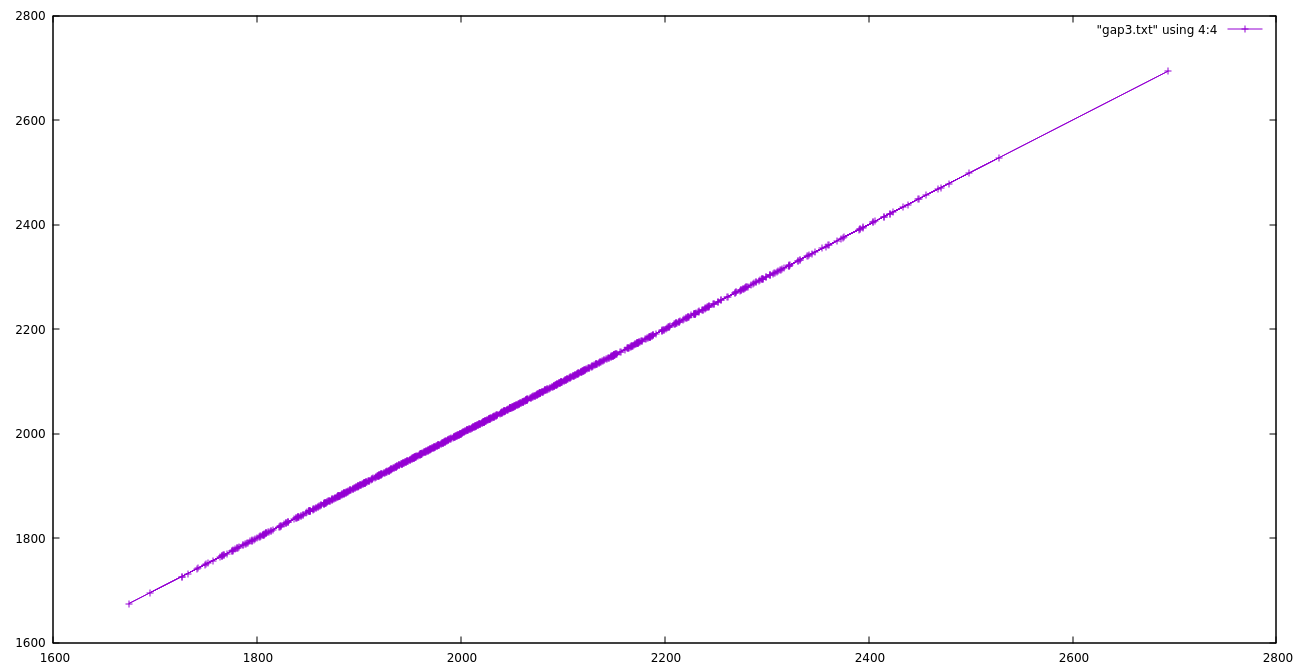
\includegraphics[scale=0.5]{imgs/gap3.png}
	\caption{Resultados de la instancia db3 con 1000 semillas}
\end{figure}


\subsection{Instancia con 40 trabajadores (db4)}
El sistema tarda un aproximado de 39 a 50 segundos para correr esta instancia con una semilla.

Ejecutar el programa con 300 semillas en esta instancia tardó 2h 23m 6s
 
Mejor Semilla: 289\\
Mejor Costo: 2123.312239567128\\
Mejor Asignación: 
\begin{lstlisting}
Trabajador 1 -> Tarea:9 , Tarea:24 , Tarea:86 , 
Trabajador 2 -> Tarea:26 , Tarea:43 , 
Trabajador 3 -> Tarea:20 , 
Trabajador 4 -> Tarea:15 , Tarea:49 , Tarea:59 , Tarea:68 , Tarea:91 , 
Trabajador 5 -> Tarea:11 , Tarea:45 , Tarea:51 , 
Trabajador 6 -> Tarea:16 , Tarea:21 , Tarea:27 , Tarea:87 , Tarea:96 , 
Trabajador 7 -> Tarea:3 , Tarea:22 , Tarea:73 , Tarea:74 , 
Trabajador 8 -> Tarea:6 , Tarea:36 , Tarea:79 , Tarea:82 , 
Trabajador 9 -> Tarea:80 , 
Trabajador 10 -> Tarea:42 , Tarea:83 , Tarea:85 , 
Trabajador 11 -> Tarea:44 , Tarea:92 , 
Trabajador 12 -> Tarea:46 , 
Trabajador 13 -> Tarea:2 , Tarea:19 , Tarea:33 , 
Trabajador 14 -> Tarea:18 , Tarea:23 , Tarea:67 , 
Trabajador 15 -> Tarea:54 , Tarea:95 , 
Trabajador 16 -> Tarea:32 , Tarea:56 , Tarea:90 , 
Trabajador 17 -> Tarea:34 , 
Trabajador 18 -> Tarea:62 , 
Trabajador 19 -> Tarea:4 , Tarea:7 , Tarea:28 , Tarea:40 , Tarea:84 , Tarea:89 , 
Trabajador 20 -> Tarea:77 , 
Trabajador 21 -> Tarea:50 , Tarea:52 , Tarea:57 , Tarea:81 , 
Trabajador 22 -> Tarea:30 , Tarea:100 , 
Trabajador 23 -> Tarea:29 , Tarea:35 , Tarea:48 , 
Trabajador 24 -> Tarea:88 , Tarea:93 , 
Trabajador 25 -> Tarea:38 , Tarea:53 , Tarea:71 , 
Trabajador 26 -> Tarea:5 , Tarea:8 , Tarea:37 , 
Trabajador 27 -> Tarea:31 , Tarea:47 , Tarea:66 , 
Trabajador 28 -> 
Trabajador 29 -> Tarea:25 , Tarea:39 , Tarea:70 , 
Trabajador 30 -> Tarea:1 , Tarea:72 , Tarea:97 , 
Trabajador 31 -> Tarea:60 , Tarea:76 , Tarea:99 , 
Trabajador 32 -> 
Trabajador 33 -> Tarea:12 , Tarea:14 , Tarea:17 , 
Trabajador 34 -> Tarea:64 , Tarea:94 , 
Trabajador 35 -> Tarea:65 , 
Trabajador 36 -> Tarea:13 , Tarea:61 , Tarea:69 , 
Trabajador 37 -> Tarea:41 , Tarea:75 , Tarea:98 , 
Trabajador 38 -> Tarea:55 , Tarea:78 , 
Trabajador 39 -> Tarea:10 , Tarea:58 , Tarea:63 , 
Trabajador 40 -> 
\end{lstlisting}

\begin{figure}[H]
	\centering
	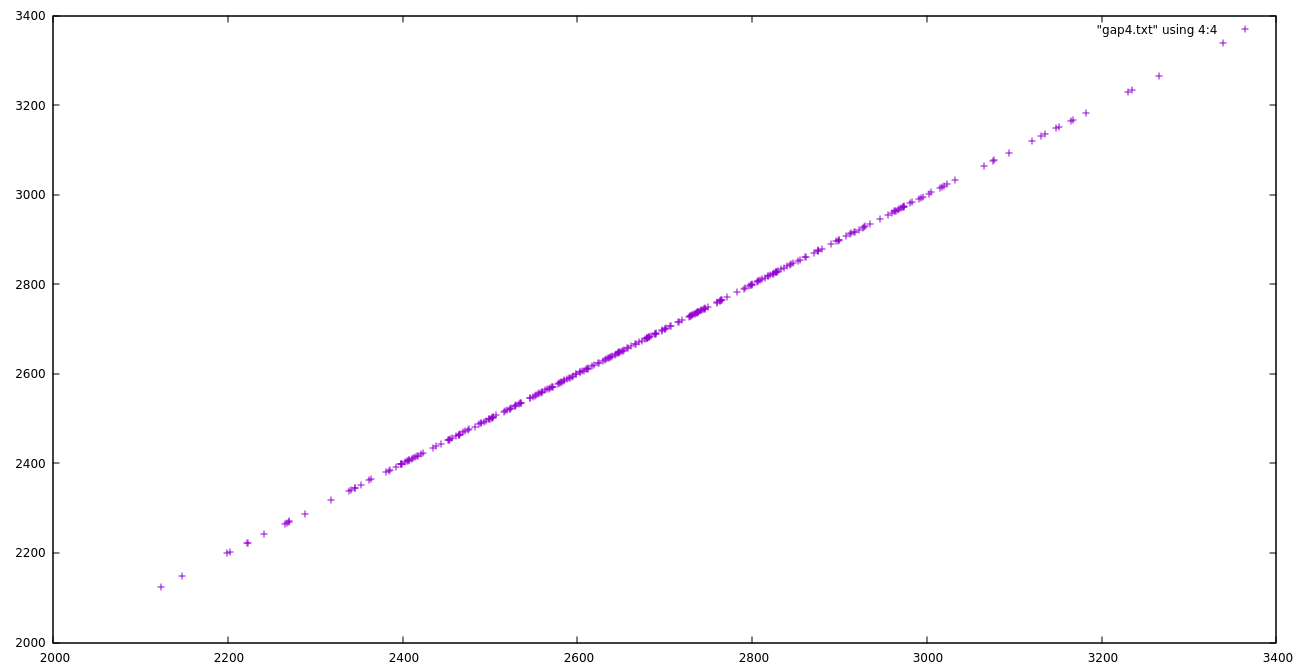
\includegraphics[scale=0.5]{imgs/gap4.png}
	\caption{Resultados de la instancia db4 con 300 semillas}
\end{figure}

\section{Conclusiones y Comentarios}

En conclusión, se hizo un proyecto que cumplía el objetivo y lo hizo de un forma bastante buena.

Tuve problemas para entender como funcionaba la heurística, tantos que en un punto decidí hacer todo con recocido simulado, pero después de leer varios artículos, en especial el de \cite{clever}, entendí una forma más sencilla de la heurística y la implementé como tal. A pesar de eso estoy satisfecha con mis resultados, mis mejores soluciones se acercaron bastantes a las del profesor y mi sistema se ejecuta en tiempo razonable.

En este proyecto estuve muchas veces en la encrucijada de si es mejor tener muchas soluciones buenas pero arriesgar a no encontrar la mejor posible o tener muchas soluciones malas con la esperanza de que la mejor pueda estar ahí. Ya que genero una solución inicial de forma greedy, estanco por así decirlo a mi sistema, debido a que va a encontrar una buena solución desde el inicio y es probable se atore en un mínimo local, la búsqueda tabú funciona justamente para ayudar con esto, pero ya que hice una implementación sencilla y para que mi sistema fuera igual de rápido que el de mis compañeros, mi heurística no recorre tanto espacio de búsqueda como para salir usualmente de estos mínimos locales. Probé ejecutar la heurística con una solución inicial aleatoria, pero no llegué a ninguna solución mejor a las que obtengo con la solución inicial greedy y tenía varias soluciones no factibles. Así que opté por mejor dar la solución inicial greedy y asegurar que la mayoría de las soluciones que se den sean factibles y bastante buenas, aunque no sean las mejores posibles.

En el futuro me gustaría retomar este proyecto y poder implementar la búsqueda tabú de forma más compleja, es decir con las memorias de mediano y largo plazo, para ver si puedo llegar a soluciones aún mejores. Así mismo sería interesante poder adaptar la búsqueda tabú en una heurística híbrida en algún futuro proyecto.

\begin{thebibliography}{9}
	\bibitem{clever}
	Brownlee J., Clever Algorithms Nature-Inspired Programming Recipes. 2011; 76-90.
	
	\bibitem{tshgap}
	Díaz Juan A., Fernández E. "A Tabu search heuristic for the generalized assignment problem". European Journal of Operational Research. 2001;132:22–38.
	  
	\bibitem{tabuglover}
	Glover F, Laguna M. "Tabu search". S.L.: Kluwer Academic; 1993.  
	
	\bibitem{gap}
	Lourenço, H.R., "Heurísticas adaptativas para el problema de
	asignación generalizada (Adaptive heuristics for the generalized assignment problem)". Proceedings of The First Spanish Congress in Evolutive and Bioinspired Algorithms. 2002;267-275
	
	\bibitem{tsgap}
	Wu Tai-Hsi, Yeh Jinn-Yi, Syau Yu-Ru. "A tabu search approach to the generalized assignment problem". Journal of the Chinese Institute of Industrial Engineers, Vol. 21, No. 3, pp. 301-311(2004)
	
	
\end{thebibliography}

Si hay duda de alguna fuente favor de contactarme para proporcionarla.

\end{document}